%%%%%%%%%%%%%%%%%%%%%%%%%%%%%%%%%%%%%%%%%%%%%%%%%%%%
% SRCs
%%%%%%%%%%%%%%%%%%%%%%%%%%%%%%%%%%%%%%%%%%%%%%%%%%%%
\section{Short Range Correlations in Nuclei}
To understand why the mean field theory fails to predict the nuclear strength and how SRCs attribute to the explanation of the missing nuclear strength, one needs to examine the modern nucleon momentum distributions which directly relate to the nucleon properties in the nucleus. While the prediction of mean field theory gives a rapid fail-off curve at momenta approaching $k_{F}$, shown in Fig.~\ref{mom_dis_ox}, experimental results~\cite{PhysRevC.53.1689} present the momentum tail with much slow falloff at $k>k_{F}$ which is similar for all nuclei from deuterium to nuclear matter. The results strongly argues again the mean field prediction, but can be easily understood if the high momentum tails are generated by the short-range part of NN interactions, i.e., SRCs.

From Fig.~\ref{potential_well}, nucleons interact at very short distance via the attractive potential which is mainly contributed by the tensor force, but their strong repulsive hard-cores prevents them to further collapse. Such dramatic processes create a correlated configuration with large relative momenta. The excitation of nucleons from these configurations significantly increase the momentum strength at $k>k_{F}$ which is not predicted by the mean field theory. However, the excitations are not related to any real excited statues of the nucleus since the total momentum of the correlated nucleons is relatively small. 
\begin{figure}[!ht]
  \begin{center}
    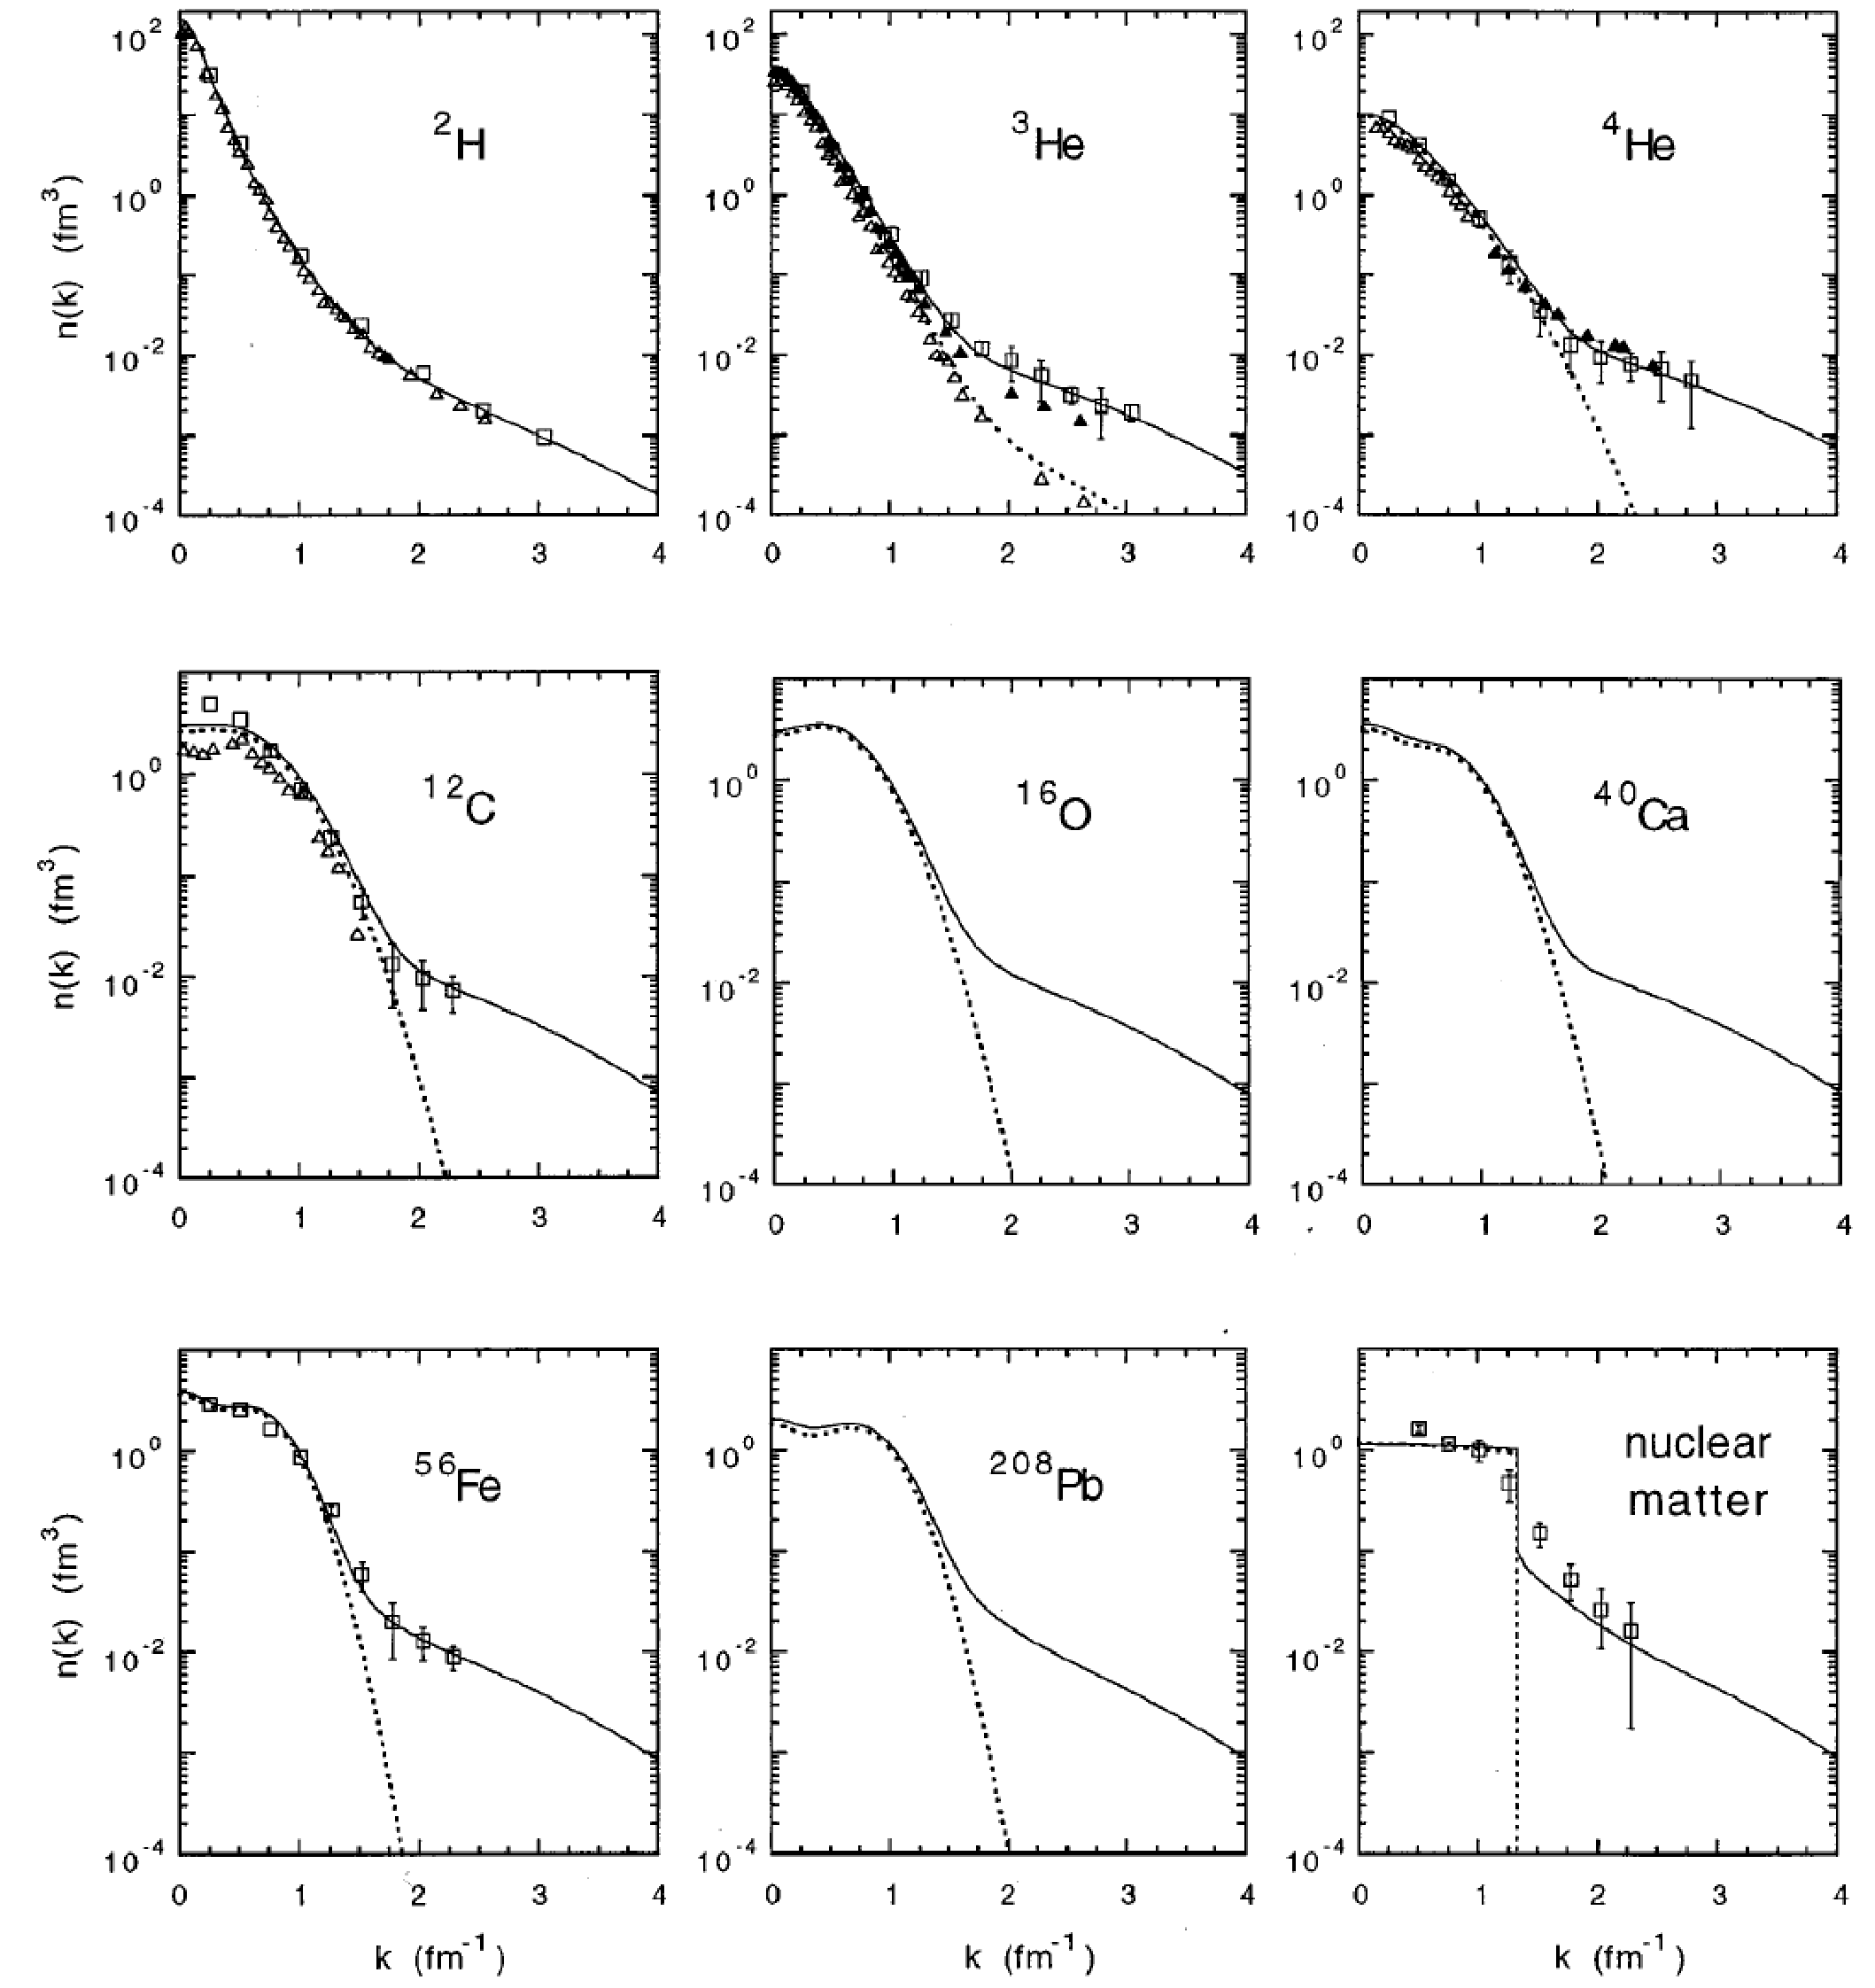
\includegraphics[type=pdf,ext=.pdf,read=.pdf,width=0.80\linewidth]{./figures/physics/Claudio_Distributions}
    \caption[Nucleon momentum distribution]{\footnotesize{Nucleon momentum distribution for various nuclei~\cite{PhysRevC.53.1689}, where dotted lines are from a mean field calculation, solid lines are from calculations involving SRCs. Dots are from experimental data.}}
    \label{mom_dis_ox}
  \end{center}
\end{figure}

In the picture of SRCs, the asymptotic form of momentum distribution can be broke down into several regions. At $k\leq k_{F}$, the strength is mainly contributed by the mean field potential. At the momentum range \emph{300 $<$ $k$ $<$ 600} MeV/c, the contribution of the mean field effect vanishes and the effect of two-nucleon short range correlation (2N-SRC) becomes dominant. The nucleons in this configuration carry large and back-to-back momenta, while the total momentum of the NN pair is negligible. Due to the fact that the NN attraction is dominated by the tensor components which produce iso-singlet pairs, i.e., $(np)_{I=0}$, one expects to see the high momentum tails of heavy nuclei to be identical to the one of deuteron, as shown in Fig.~\ref{mom_dis_ox}. The configuration of 2N-SRC breaks down at much higher momentum limit (\emph{600 $\leq$ $k$ $\leq$ 800} MeV/c) where the isospin-independent repulsive core begins to dominate, and the inclusion of three-nucleon short range correlation (3N-SRC) should be manifested~\cite{src_john}. At extremely high $k$ limit where the nucleon kinetic energy is comparable with the excitation energy of nucleons, non-nucleonic degree-of-freedom may be needed to be considered~\cite{src_john}.
\begin{figure}[!ht]
  \begin{center}
    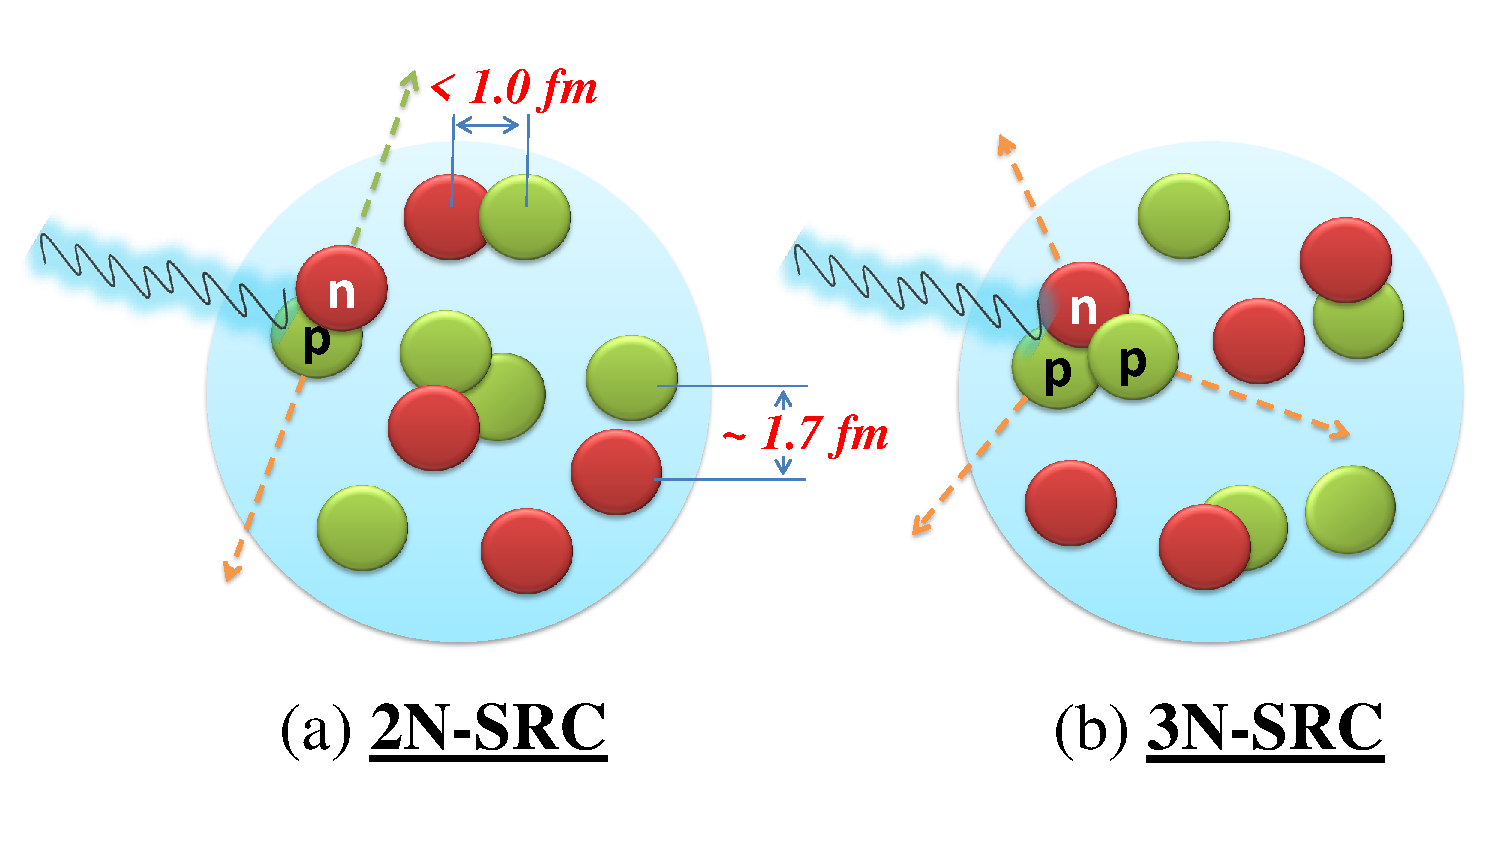
\includegraphics[type=pdf,ext=.pdf,read=.pdf,width=0.80\linewidth]{./figures/physics/2NSRC3NSRC}
    \caption[Diagrams of 2N- and 3N-SRC]{\footnotesize{Diagram of 2N- and 3N-SRC. On the left diagram the virtual phone breaks up the 2N-SRC pair in back-to-back ejection, and on the right diagram the break-up of 3N-SRC configuration results in correlated nucleon ejecting in different direction so their total momentum remains at zero.}}
    \label{2nsrc3nsrc}
  \end{center}
\end{figure}

\subsection{Two-Nucleon Correlations}
Based on the discussion above, the dominance of 2N-SRC in the nucleus at $k>k_{F}$ should yield an momentum distribution proportional to the one in deuterium:
\begin{equation}
  n_{A}(k) = a_{2}(A,Z)\cdot n_{D}(k), \qquad for\quad k>k_{F},
  \label{2nsrc_mon_scaling}
\end{equation}   
where $n_{D}(k)$ denotes the momentum distribution of deuterium and $a_{2}(A,Z)$ relates to the probability of finding such two-nucleon configuration in the nucleus with nuclear number $A$ and proton number $Z$. One can study the scaling of $a_{2}$ as the function of \emph{k}, by taking ratio of momentum distribution of different nuclei to deuterium, $n_{A}(k)/n_{D}(k)$.

The momentum distribution can be reconstructed from the ground state wave-function but is not an experimental observable. Instead, one studies SRCs through the spectral function which directly relates to the cross section of physical processes (Eq~\ref{quasi_xs_spectral_function}). In IPSM, one can define the spectral function as~\cite{Frankfurt_misak}:
\begin{equation}
  S_{A}(E_{R},p_{i}) = |<\phi_{A-1}|\delta(-p_{i}^{2}/(2m_{A-1}) + E_{R}-E_{m})a(k)|\psi_{A}>|^{2}, 
  \label{spectral_2nsrc}
\end{equation}
which represents a product of the probability of finding a nucleon in the nucleus with initial momentum $p_{i}$, and the probability of the residual system carrying recoil energy $E_{R}$ after the removal of this nucleon. \emph{a(k)} denotes an operator to remove a nucleon from the nucleus A, $E_{m}$ depends on A and represents the excitation energy of the $A-1$ system at rest, and $-p_{i}^{2}/(2m_{A-1})$ is the kinetic energy of the center of mass. 

When a nucleon in the 2N-SRC configuration is instantly knocked out by a high energy probe, its paired nucleon with an equal momentum is rejected in the opposite direction, while the $A-2$ residual nucleus remains unperturbed ($E_{m}\sim 0$). When only the knock-out nucleon is interested, the kinetic energy of the correlated nucleon is shared by the entire $A-1$ system. From Eq~\eqref{spectral_2nsrc}, the average recoil energy of the $A-1$ system can be approximately given as:
\begin{equation}
  <E_{R}>_{2N-SRC} \sim \frac{p^{2}_{i}}{2m_{N}}.
  \label{Er_2nsrc}
\end{equation}

Since $E_{R}$ directly relates to the initial momentum of the nucleon in 2N-SRC, and the spectral function links to the momentum distribution (Eq.~\eqref{np_mom_eq}), observation of the correlation between the spectral function and $E_{R}$ enables one to examine the contribution of SRCs but however, it is not uniquely sensitive to SRCs. Indeed, any processes that involving NN interaction, such as meson exchange currents,yields the same result in Eq~\eqref{Er_2nsrc}. One can check the dominance of the SRCs by applying additional kinematic conditions to suppress long range NN interactions, which will be discussed in next section.

\subsection{Three-Nucleon Correlations}
Similar to the deuterium-like configuration of the 2N-SRC pair, the momentum distribution of a nucleon in a 3N-SRC configuration should be identical to the case in $^{3}H$ (pnn) and $^{3}He$ (ppn). For example,
\begin{equation}
  n_{A}(k) = a_{3}(A,Z)\cdot n_{^{3}He}(k), \qquad for\quad k>800 \quad MeV/c,
  \label{3nsrc_mon_scaling}
\end{equation}  
where similarly, $n_{^{3}He}(k)$ is the momentum distribution of $^{3}He$ and $a_{3}(A,Z)$ is the probability of finding three-nucleon configuration in the nucleus $A$. 
\begin{figure}[!ht]
  \begin{center}
    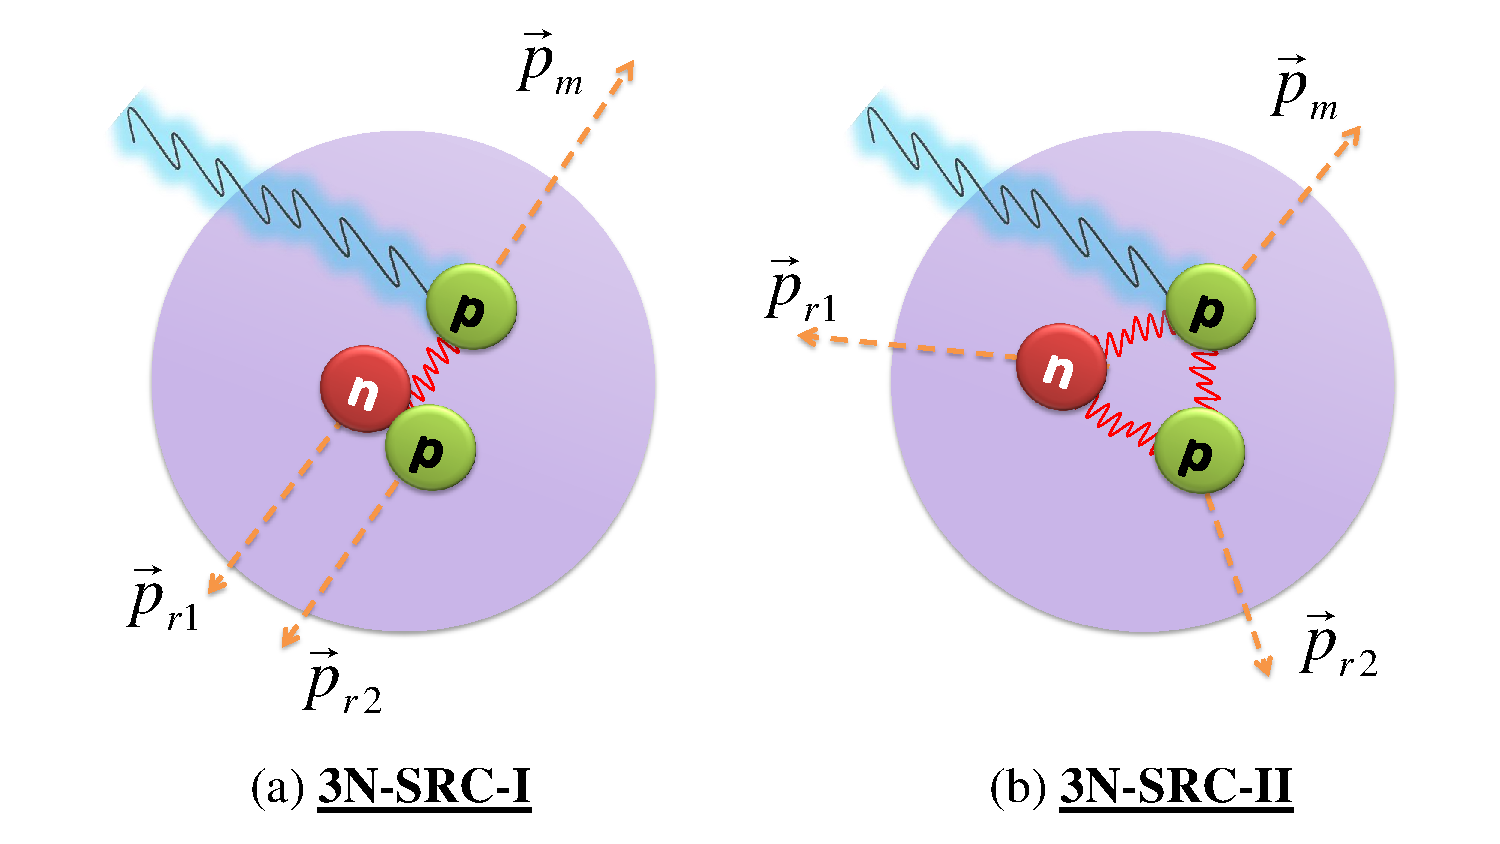
\includegraphics[type=pdf,ext=.pdf,read=.pdf,width=0.80\linewidth]{./figures/physics/3nsrc_two_types}
    \caption[Two types of 3N-SRC configuration]{\footnotesize{Two types of 3N-SRC configuration~\cite{Frankfurt_misak}.}}
    \label{3nsrc_two_types}
  \end{center}
\end{figure}

However, the configuration of 3N-SRC is more complicated compared with the simple back-to-back picture of 2N-SRC. In general, there are two types of 3N-SRC, as shown in Fig.~\ref{3nsrc_two_types}. The first type, namely 3N-SRC-I, is the situation of two nucleons share the initial momentum which is equal to the struck nucleon but in the opposite direction, a configuration similar to 2N-SRC but involving three nucleons. The effect of 3N-SRC-I typically dominates at $p_{i}\geq 600 MeV/c$ with the average recoil energy of the $A-2$ residual system:
\begin{equation}
  <E_{R}>_{3N-SRC-I} \sim \frac{p^{2}_{i}}{4m_{N}}.
  \label{Er_3nsrc_1}
\end{equation}
which is approximately equal to one half of the recoil energy in 2N-SRC. This configuration gives the major contribution in the kinematic region of 3N-SRC.

The second type, 3N-SRC-II, refers to the configuration of three nucleon carrying momenta all exceeding the Fermi momentum in three different direction, and the average recoil energy of the residual system in this configuration is:
\begin{equation}
  <E_{R}>_{3N-SRC-II} \sim \frac{p^{2}_{i}}{m_{N}},
  \label{Er_3nsrc_2}
\end{equation}
which is larger than the average recoil energy of 3N-SRC-I, indicating the probability of 3N-SRC-II is more rare than the one of 3N-SRC-I, although the former one is easier to be observed experimentally. 

Eq~\eqref{Er_2nsrc}, Eq~\eqref{Er_3nsrc_1} and Eq~\eqref{Er_3nsrc_2} reveal that the average recoil energy of 2N-SRC is in between the two average recoil energies of 3N-SRC, and for 2N-SRC the distribution of $E_{R}$ as a function of $p_{i}$ is very broad, so its capability of identifying contributions from 2N-SRC and 3N-SRC to the spectral function is limited. New kinematic quantities are needed to separate these two processes, and are introduced next.

\subsection{Relativistic Approach}
The high energy process of knocking out short range correlated nucleons with very high momenta make one more naturally to apply the study of SRCs in the relativistic regime. A relativistic projectile moving along the z-direction probe the light-cone (LC) wave-function of the nucleus, $\psi_{A}(\alpha_{1},k_{1,t},...,\alpha_{i},k_{i,t},...,\alpha_{A},k_{A,t})$, where the LC variable is defined as~\cite{Frankfurt_misak}:
\begin{equation}
  \alpha_{i} = A\left(\frac{E_{i}-p_{i,z}}{E_{A}-p_{A,z}}\right)=A\left(\frac{E_{i}^{lab}-p_{i,z}^{lab}}{M_{A}}\right),
\end{equation}  
where ($E_{i}-p_{i,z}$) and ($E_{A}-p_{A,z}$) are the initial energy and longitudinal momentum of constituent nucleons and the target nucleus, $A$, respectively. $\alpha_{i}$ is invariant under Lorentz boosts in the z-direction. In the rest frame of the nucleus, $E_{A}-p_{A,z}=M_{A}$, where $M_{A}$ is the nuclear mass. 

Similar to the definition of $x_{bj}$ in inelastic scattering (Eq~\ref{xbj_define}), $\alpha_{i}$ denotes the LC fraction of the nucleus momentum carried by the nucleon, hence $\sum_{i}^{A}\alpha_{i}=A$. While $\alpha_{i}\leq 1$ limits the momentum fraction of the nucleon carried by the quark, to have $\alpha_{i}>1$ requires at least two nucleons involved in the scattering. Furthermore, three nucleons are required to share their momentum to have $\alpha_{i}>2$. $\alpha_{i}$ consequently becomes an ideal variable to distinguish between 2N-SRC and 3N-SRC. Considering the energy and momentum conservation law for the nucleon knock-out with a virtual photon from the nucleus, one can rewrite the LC variable as~\cite{src_john}:
\begin{equation}
  \alpha_{i}=x_{bj}\left(1+\frac{2p_{i,z}}{\nu+|\mathbf{q}|}\right)+\frac{W_{N}^{2}-m_{i}^{2}}{2m_{i}\nu},
  \label{alpha_xbj}
\end{equation}
where $\nu$ and $\mathbf{q}$ is the energy and momentum transfer of the virtual photon, respectively, and $W_{N}^{2}=(\mathbf{p_{i}}+\mathbf{q})^{2}$. For the quasi-elastic process, $W_{N}\simeq m_{i}$ yields a simple connection between $\alpha_{i}$ and $x_{bj}$. At sufficiently large $Q^{2}$, $\alpha_{i}$ is usually replaced by $x_{bj}$: 
\begin{equation}
  \alpha_{i}\rightarrow x_{bj}, 
\end{equation}
when $Q_{2}\rightarrow \infty$. However, these two variables have distinct differences for $Q^{2}$ values in few $GeV^{2}$ range. One needs to examine the different scaling of SRCs as a function of $x_{bj}$ and $\alpha_{i}$ at the region of low $Q^{2}$ values. 	
\subsection{Isospin Effect}
\begin{figure}[!ht]
  \begin{center}
    \includegraphics[type=pdf,ext=.pdf,read=.pdf,width=0.80\linewidth]{./figures/physics/mom_dis_np}
    \caption[Momentum distribution for proton and neutron and their ratio]{\footnotesize{Left: Momentum distribution for proton (solid) and neutron (dashed) in $^{3}He$; Right: Ratio of proton to neutron momentum distribution. Plots were originally from~\ref{src_john}.}}
    \label{mom_dis_np}
  \end{center}
\end{figure}   
Early analysis assumed the isospin-independence of SRCs, which means that the ratio of neutrons to protons in SRCs is equal to the $N/Z$ ratio of the nucleus. However, numerical studies~\cite{PhysRevC.72.054310} and results from experiments~\cite{Subedi:2008zz} reveal that the tensor interaction dominates the attractive potential of 2N-SRC. Accordingly, one expects that 2N-SRC pairs should be mainly in iso-singlet ($np,~T=0$) states. The iso-triplet ($pp$,$np$ and $nn$, $T=1$) pairs can be close together without interacting strongly until their repulsive forces become strong~\cite{src_john}.

Fig.~\ref{mom_dis_np} shows a calculation of the momentum distribution for protons and neutrons and their ratio in $^{3}He$~\cite{Pieper_Wiringa}. In the assumption of isospin-independence, the momentum ratio of protons to neutrons should be equal to two, but if the SRCs are isospin-dependent, the ratio becomes one when SRCs dominate at $k>k_{F}$. The left plot gives the value of the ratio at $k>k_{F}$ roughly equal to 1.5, which suggests that the isospin effect largely deviates from the assumption of isospin independence. The reason why $np_{T=0}$ configuration does not totally dominates is that the $T=1$ channels are not completely suppressed, especially at very large momentum, where the configuration of 3N-SRC is more complicated. Another calculation~\cite{PhysRevLett.98.132501} extended the study to other nuclei provides the similar results. Shown in Fig.~\ref{isospin_src}, the momentum distribution of $np$ pairs is much more significant than one of the $pp$ pairs at $300<k<600$ $MeV/c$.
\begin{figure}[!ht]
  \begin{center}
    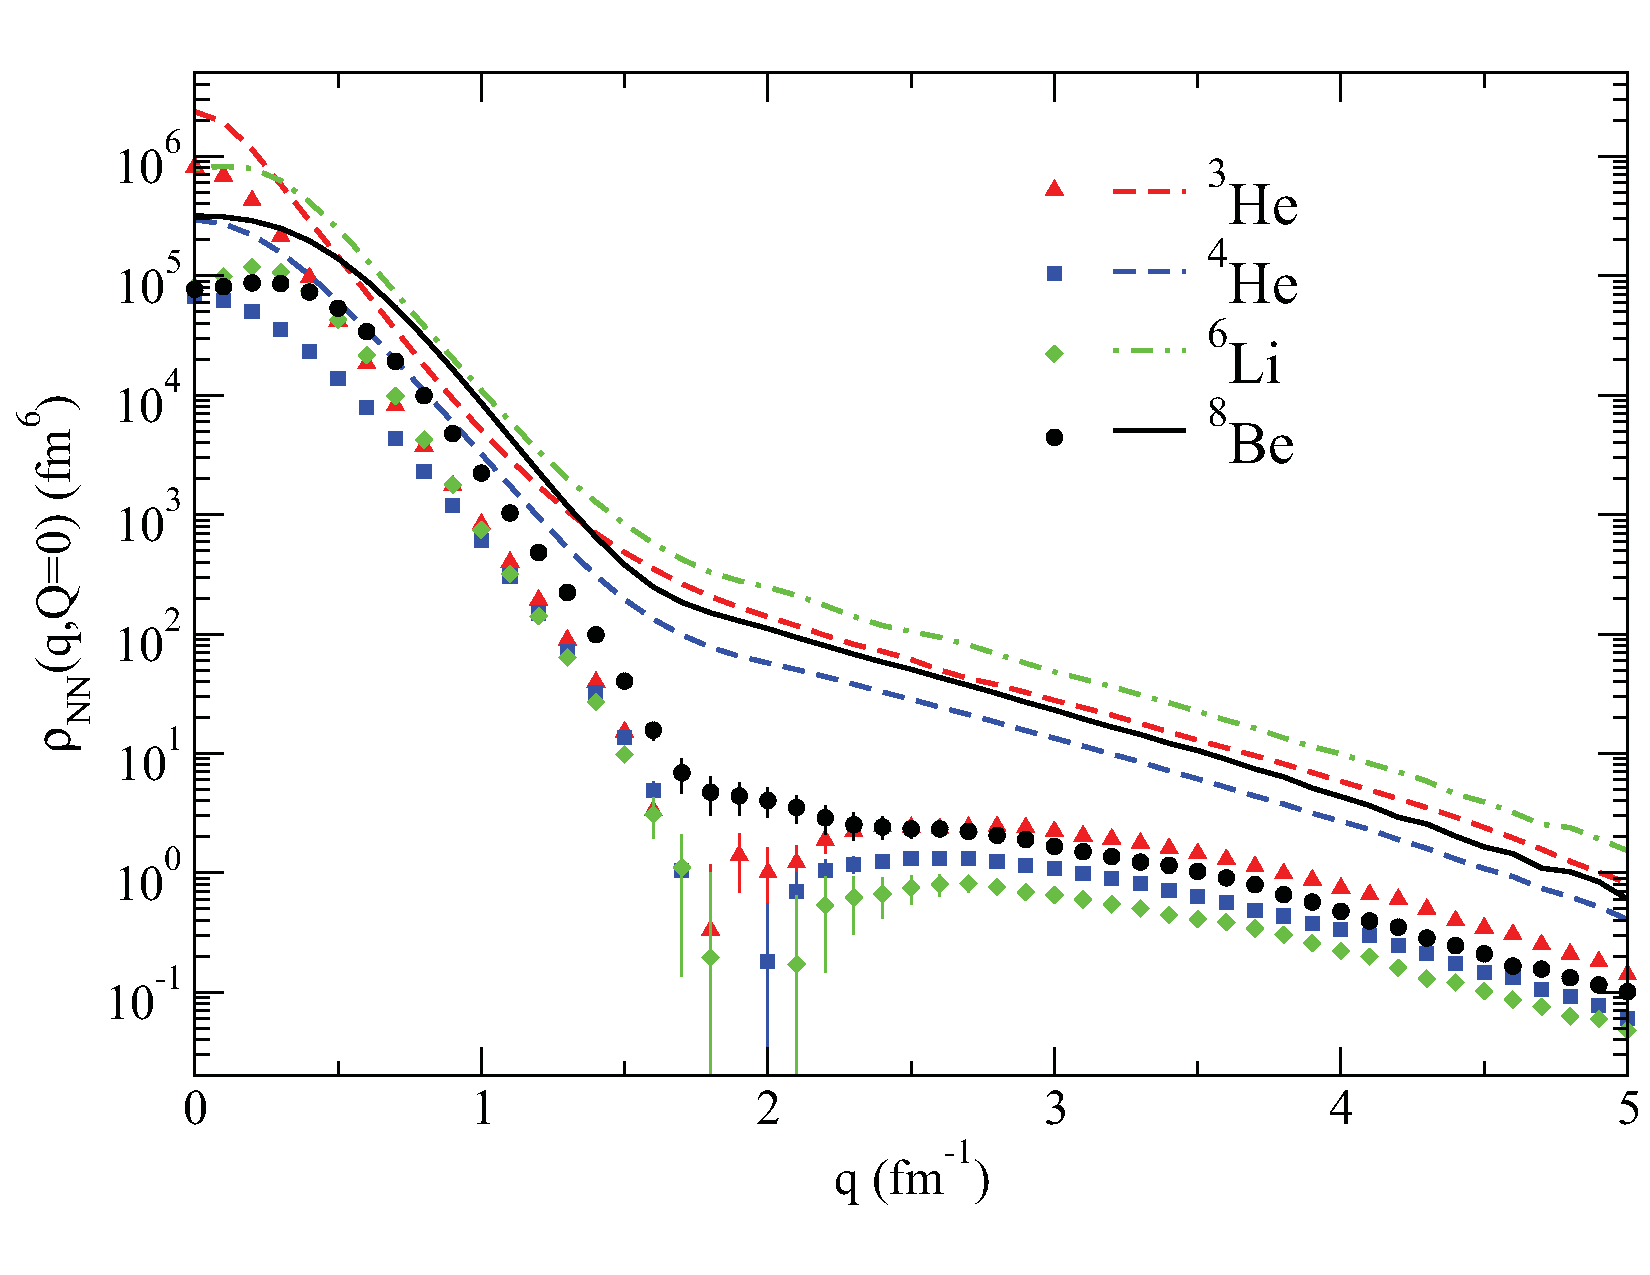
\includegraphics[type=pdf,ext=.pdf,read=.pdf,width=0.60\linewidth]{./figures/physics/isospin_src}
    \caption[Isospin effect in momentum distribution]{\footnotesize{Isospin effect in momentum distribution, where lines represents the momentum distribution in $np$ and dots represents the momentum distribution in $pp$. The dip in the $pp$ momentum distribution around 2 $fm^{-1}$ is due to the tensor correlations of protons~\cite{src_john,PhysRevLett.98.132501}.}}
    \label{isospin_src}
  \end{center}
\end{figure} 

The isospin effect in 2N-SRC can be studied by triple-coincidence experiments, which not only measures the scattered electrons and the struck protons in a 2N-SRC configuration but also simultaneously detects protons and neutrons rejected in the opposite direction with equal momentum. Inclusive cross sections is also sensitive to such effect. One can examine the isospin-dependence by measuring the cross section ratio of two isotopes in the SRCs region, such as $^{48}Ca/^{40}Ca$~\cite{e08014_pr} and $^{3}He/^{3}H$~\cite{E12_11_112_pr}.

\section{Probing SRCs}
To isolate the high momentum nucleons and perform clean measurements of SRCs in nuclei, one needs to carefully selecting the proper kinematics settings to suppress other competing processes during scattering. By isolating the process of a high energy probe instantly removing a nucleon from SRCs, one is able to extract reliable information on the spectral function and momentum distribution from the measured observables. 

\subsection{Kinematics Conditions}
Although there are different kinds of reactions for probing SRCs, there share the common kinematic conditions to provide a clean study. Overall, the desire to instantly remove the nucleon from the SRCs can be achieved by requiring sufficiently large energy and momentum transfer scales which significantly exceed the excitation scale of the nucleus~\cite{Frankfurt1981215,Frankfurt_misak}
\begin{equation}
  \nu >> V_{NN}, \qquad |\mathbf{q}| >> m_{N}/c,
  \label{src_condition1}
\end{equation}
where $V_{NN}$ is the characteristic potential of the NN interaction and $m_{N}$ is the nucleon mass. A reaction removing a nucleon from the nucleus under this condition allows the residual system to remain intact, where the spectral function will directly reflect the properties of SRCs~\cite{src_john}.

The contribution of long range interactions, such as MECs, is suppressed by a factor of $Q^{-4}$ with respect to the production of SRCs, and can be generally suppressed by requiring~\cite{M_Sargsian_JPG_29_2003}:
\begin{equation}
  Q^{2} > 1.0~GeV^{2} >> m_{meson}^{2}.
  \label{src_condition2}
\end{equation}
In this condition, intermediate state resonances, such as the isobars current (IC), still have sizeable contributions. For example, for $1~GeV^{2}<Q^{2}<4~GeV^{2}$, $\gamma N\rightarrow \Delta$ transition is comparable with $\gamma N\rightarrow N$. Those resonance states are generally within the region of $0<x_{bj}<1$, and their contributions can be suppressed by working at the region above the quasi-elastic scattering:
\begin{equation}
  x_{bj} > 1.
  \label{src_condition3}
\end{equation}

\begin{figure}[!ht]
  \begin{center}
    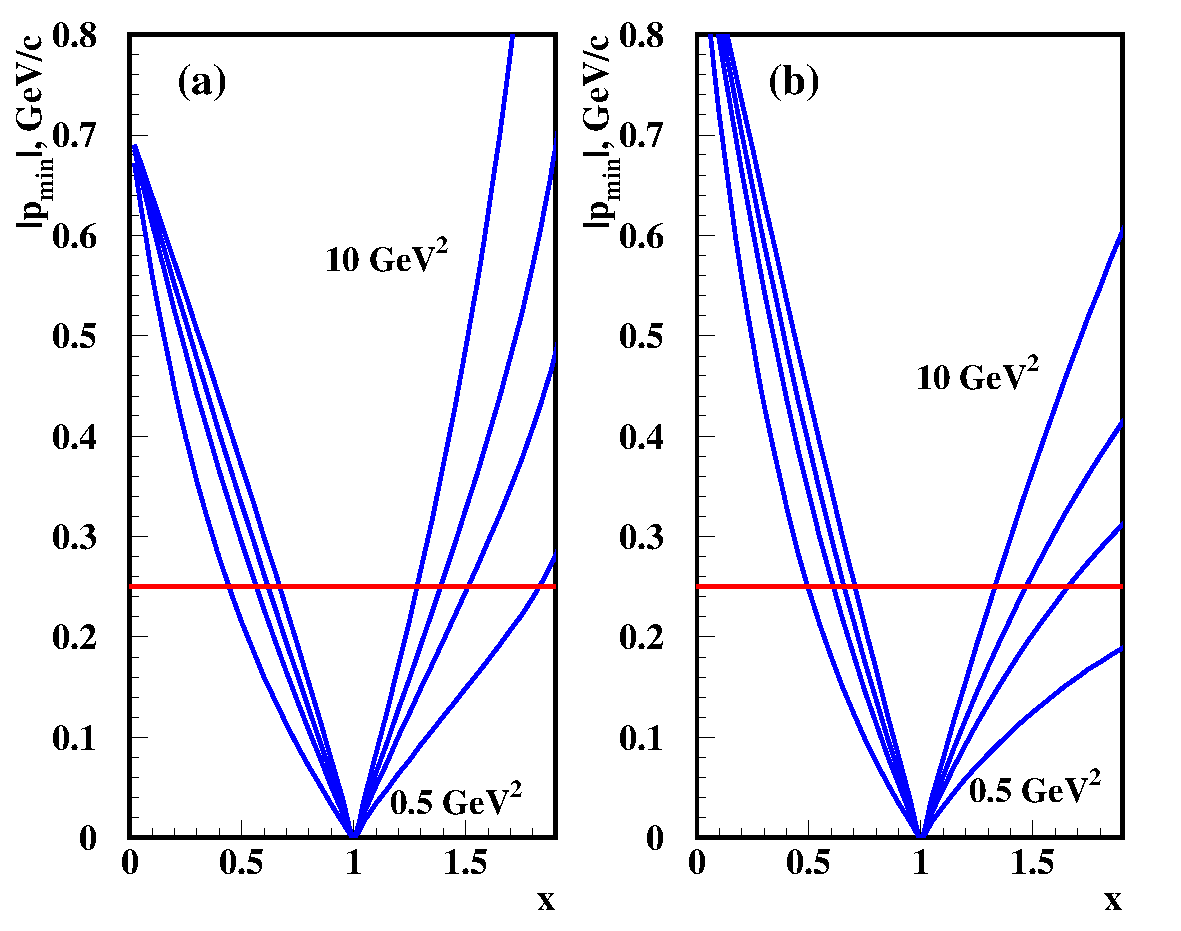
\includegraphics[type=pdf,ext=.pdf,read=.pdf,width=0.60\linewidth]{./figures/physics/p_min_x}
    \caption[Minimum momentum of the struck nucleon as function of $x_{bj}$ and $Q^{2}$]{\footnotesize{Minimum momentum of the struck nucleon as function of $x_{bj}$ and $Q^{2}$ for scattering off a nucleon from deuterium (right) and from gold (right), where the values of $Q^{2}$ from bottom to top are 0.5, 1.5, 3.0 and 10 $GeV^{2}$, respectively~\cite{Frankfurt_misak, src_john}. The red line sets the value of the Fermi momentum ($k_{F}$). These plots indicate that heavy nuclei require higher values of $Q^{2}$ and $x_{bj}$ to reach the Fermi momentum and fully suppress the mean field contribution.}}
    \label{kin_cond_q2_xbj}
  \end{center}
\end{figure} 
Fig.~\ref{kin_cond_q2_xbj} demonstrates that the combination of kinematic conditions (Eq~\eqref{src_condition2} and Eq~\eqref{src_condition3}). When $Q^{2}$ value is not sufficiently large ($\sim 0.5~GeV^{2}$) for scattering off nucleons from deuterium, the 2N-SRC production is almost suppressed by other processes even at very higher $x_{bj}$ ($\sim 1.8$). At very high $Q^{2}$ ($\sim 10~GeV^{2}$), the minimum momentum requirement of the struck nucleon easily achieves at relatively low $x_{bj}$ ($\sim 1.3$) due to the highly suppression of mean field effect. For heavy nuclei, the requirement of $x_{bj}$ and $Q^{2}$ is much more strict to reach the Fermi momentum. 

Together with Eq~\eqref{src_condition1}, those kinematic conditions enable the clean measurement of high momentum nucleons from SRCs and meanwhile, largely eliminate the contribution from mean field effect, such as MECs and IC.

\subsection{Inclusive Measurement}
The inclusive cross section measurement of $A(e,e')$ reaction in quasi-elastic region was first applied to isolate SRCs and currently is the only way to probe 3N-SRC. The cross section for $x>1.3$ and $Q^{2}>1~GeV^{2}$ is written as~\cite{Frankfurt1988235}:
\begin{eqnarray}
  \sigma_{A}(x_{bj},Q^{2}) &=& \sum_{j=2}^{A}\frac{A}{j} a_{j}(A) \sigma_{j}(x_{bj},Q^{2}) \nonumber \\
  &=& \frac{A}{2}a_{2}(A)\sigma_{2}(x_{bj},Q^{2})+\frac{A}{3}a_{3}(A)\sigma_{3}(x_{bj},Q^{2})+...,
  \label{xs_src_inclusive}
\end{eqnarray}
where $\sigma_{j}$ is the cross section for scattering from a $j$-nucleon correlation and $a_{j}(A)$ denotes the probability of finding a nucleon in this correlation. First two terms represents the contributions from 2N-SRC and 3N-SRC. 

From Eq~\eqref{2nsrc_mon_scaling} and Eq~\eqref{3nsrc_mon_scaling}, 2N-SRC (3N-SRC) predicts the scaling of the nucleon momentum distribution for heavy nucleus $A$ with respect to the deuterium ($^{3}He$). In the region of $1.3<x_{bj}<2.0$ where 2N-SRC dominates, $a_{2}(A)$ can also be given by the cross section ratio:
\begin{equation}
  a_{2}(A) = \frac{2}{A}\frac{\sigma_{A}(x_{bj},Q^{2})}{\sigma_{D}(x_{bj},Q^{2})},
  \label{src_a2}
\end{equation}
where $\sigma_{D}(x_{bj},Q^{2})$ is the cross section for scattering from the deuterium target. $a_{2}(A)$ is identical to the one defined in Eq~\eqref{2nsrc_mon_scaling} and the formula indicates that at 2N-SRC region, the value of $a_{2}$ is independent of $x_{bj}$ and $Q^{2}$, but only relates to the nuclear number. The value of the ratio on the scaling plateau directly gives the relative number of 2N-SRC pairs in the nucleus.
\begin{figure}[!ht]
  \begin{center}
    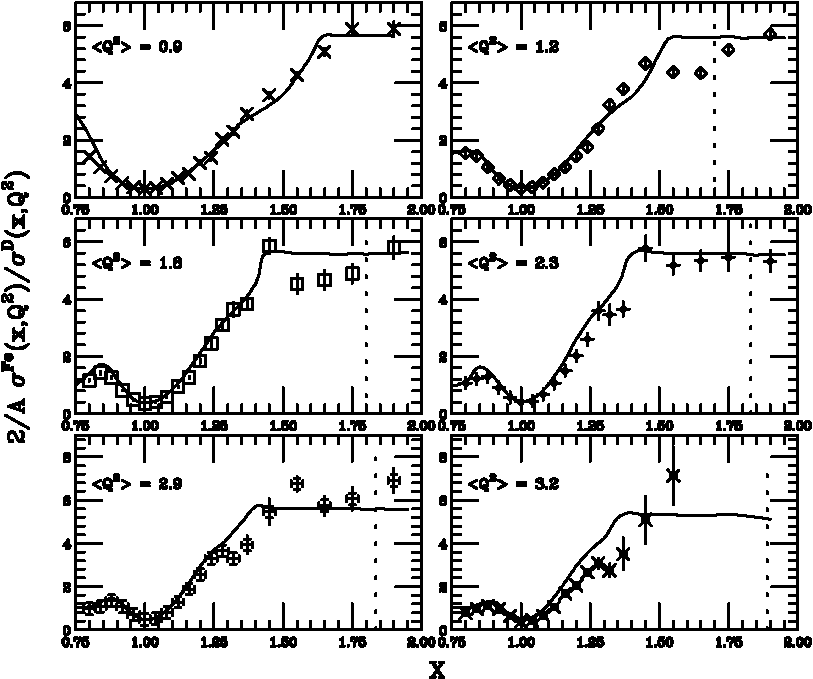
\includegraphics[type=pdf,ext=.pdf,read=.pdf,width=0.60\linewidth]{./figures/physics/SLAC_2NSRC_First}
    \caption[First evidence of 2N-SRC from SLAC]{\footnotesize{First evidence of 2N-SRC from SLAC~\cite{SLAC_Measurement_PRC.48.2451}. Y-axis is the cross section ratio of $^{56}Fe$ to $^{2}H$ for $Q^{2}=1.2-2.9~GeV^{2}$ and x-axis is $x_{bj}$. The plateau of 2N-SRC clearly is clearly showed at $x_{bj}>1.5$ and agrees with the theoretical prediction based on the 2N-SRC model (lines).}}
    \label{slac_2nsrc_first}
  \end{center}
\end{figure}

Fig.~\ref{slac_2nsrc_first} shows the experiment results from SLAC~\cite{SLAC_Measurement_PRC.48.2451}, which for the first time observed such a plateau using the cross section ratio of $^{56}Fe$ to $^{2}H$ at $x_{bj}>1.5$ and $Q^{2}=1.2-2.9~GeV^{2}$. However, the statistics were limited and the deuterium data were taken at different kinematics, so the result was extracted with nontrivial extrapolations. Recent Jefferson Lab results from Hall-B using Large Acceptance Spectrometer (CLAS)~\cite{PhysRevLett.96.082501} and from E02-019 data in Hall-C~\cite{PhysRevLett.108.092502} studied the values of $a_{2}$ for various nuclei with higher statistics and with better resolution, and both results show sound agreement at the 2N-SRC region (Fig.~\ref{CLAS_2NSRC_3NSRC} and Fig.~\ref{E02019_2NSRC_3NSRC}). 

Similarly, one can study 3N-SRC at $2<x_{bj}<3$ with the cross section ratio of the heavy nucleus to $^{3}He$:
\begin{equation}
  a_{3}(A) = K\cdot\frac{3}{A}\frac{\sigma_{A}(x_{bj},Q^{2})}{\sigma_{^{3}He}(x_{bj},Q^{2})},
  \label{src_a3}
\end{equation}
which is the same as the one in Eq~\eqref{2nsrc_mon_scaling} and denotes the number of $^{3}He$-like 3N-SRC configuration in the nucleus. $K$ is a kinematic constant to correct difference of the electron-proton and electron-neutron cross sections:
\begin{equation}
  K = \frac{\sigma_{ep}+\sigma_{en}}{Z\sigma_{ep}+(A-Z)\sigma_{en}}.
\end{equation}
\begin{figure}[!ht]
  \begin{center}
    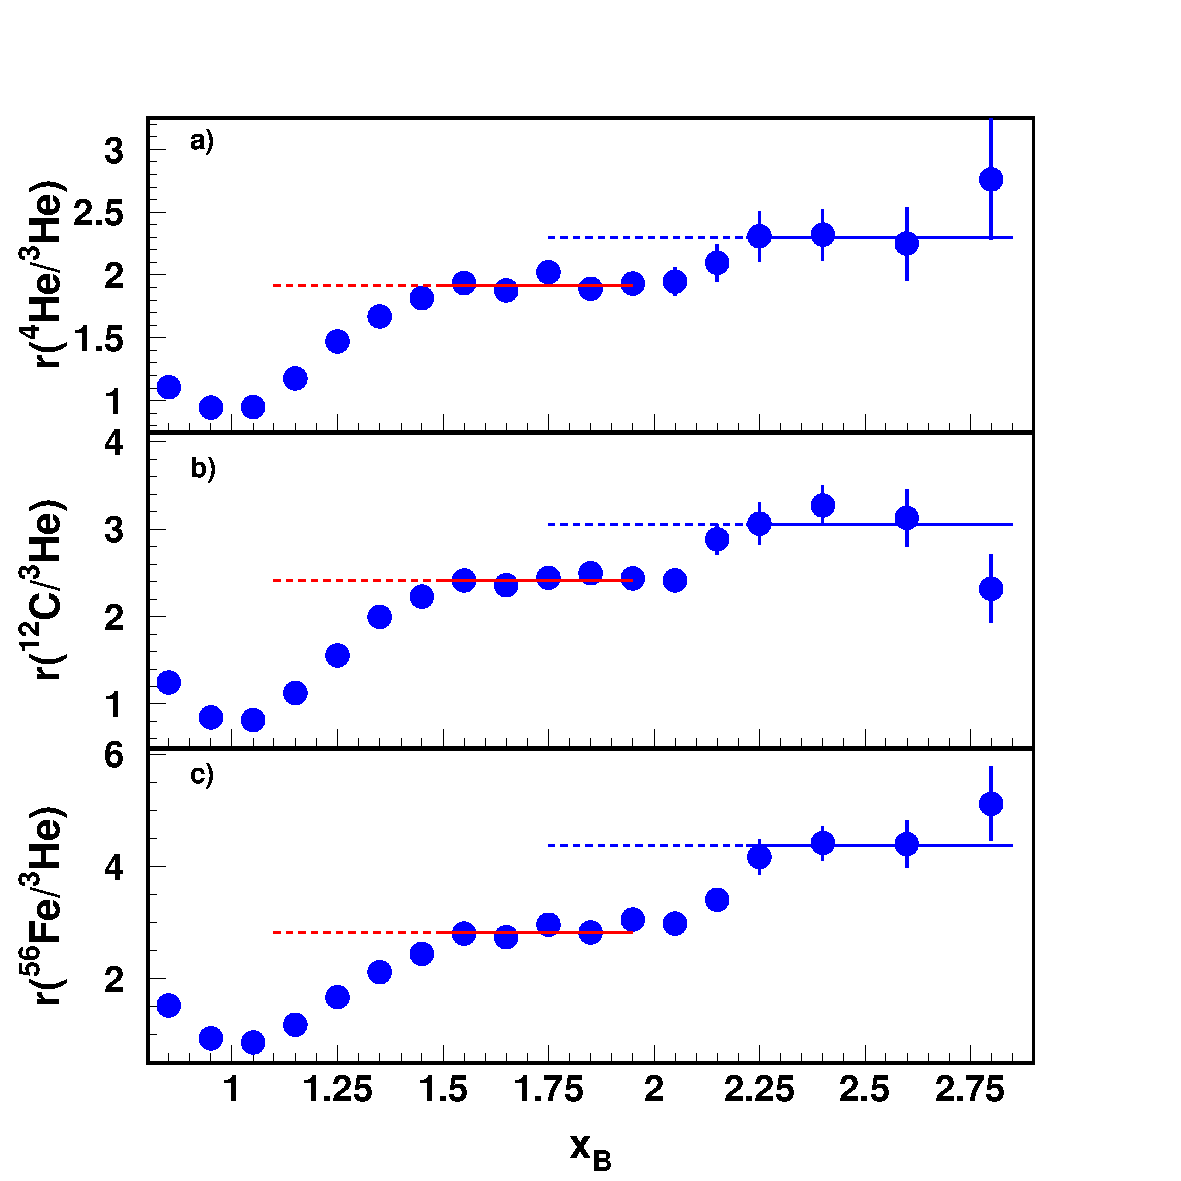
\includegraphics[type=pdf,ext=.pdf,read=.pdf,width=0.60\linewidth]{./figures/physics/CLAS_2NSRC_3NSRC}
    \caption[2N-SRC and 3N-SRC results from Hall B]{\footnotesize{2N-SRC and 3N-SRC results from Hall B~\cite{PhysRevLett.96.082501}. The top, middle and bottom plots give the cross section ratios of $^{4}He$, $^{12}C$ and $^{56}Fe$ to $^{3}He$, respectively. In each plot, both the 2N-SRC plateau (in $1.5<x_{bj}<2$) and the 3N-SRC plateau (in $x_{bj}>2$) can be observed.}}
    \label{CLAS_2NSRC_3NSRC}
  \end{center}
\end{figure} 

The CLAS data for the first time measured the kinematic region of 3N-SRC and observed the plateau raises at $x_{bj}>2.3$. The E02-019 data, however, yields a different result in this region. From Fig.~\ref{E02019_2NSRC_3NSRC}, the cross section ratio of $^{4}He/^{3}He$ reaches the scaling region slightly later than the CLAS result ($x_{bj}>2.5$). And the scaling plateau can not be conformed due to the large error bars, mainly because of the large statistical subtraction to remove the contamination from the aluminium windows. A simple interpolation of the discrepancy is impossible since two experiments ran at very different $Q^{2}$ range ($Q^{2}\sim 1.6~GeV^{2}$ for CLAS and $Q^{2}\sim 2.7~GeV^{2}$ for E02-019). It is not clear that both measurements were able to isolate the 3N-SRC contributions. The new experiment in Hall-A, E08-014, focuses on studying the scaling of 3N-SRC at $x_{bj}>2$ with much better accuracy, and the new preliminary results will be presented in this thesis. 
\begin{figure}[!ht]
  \begin{center}
    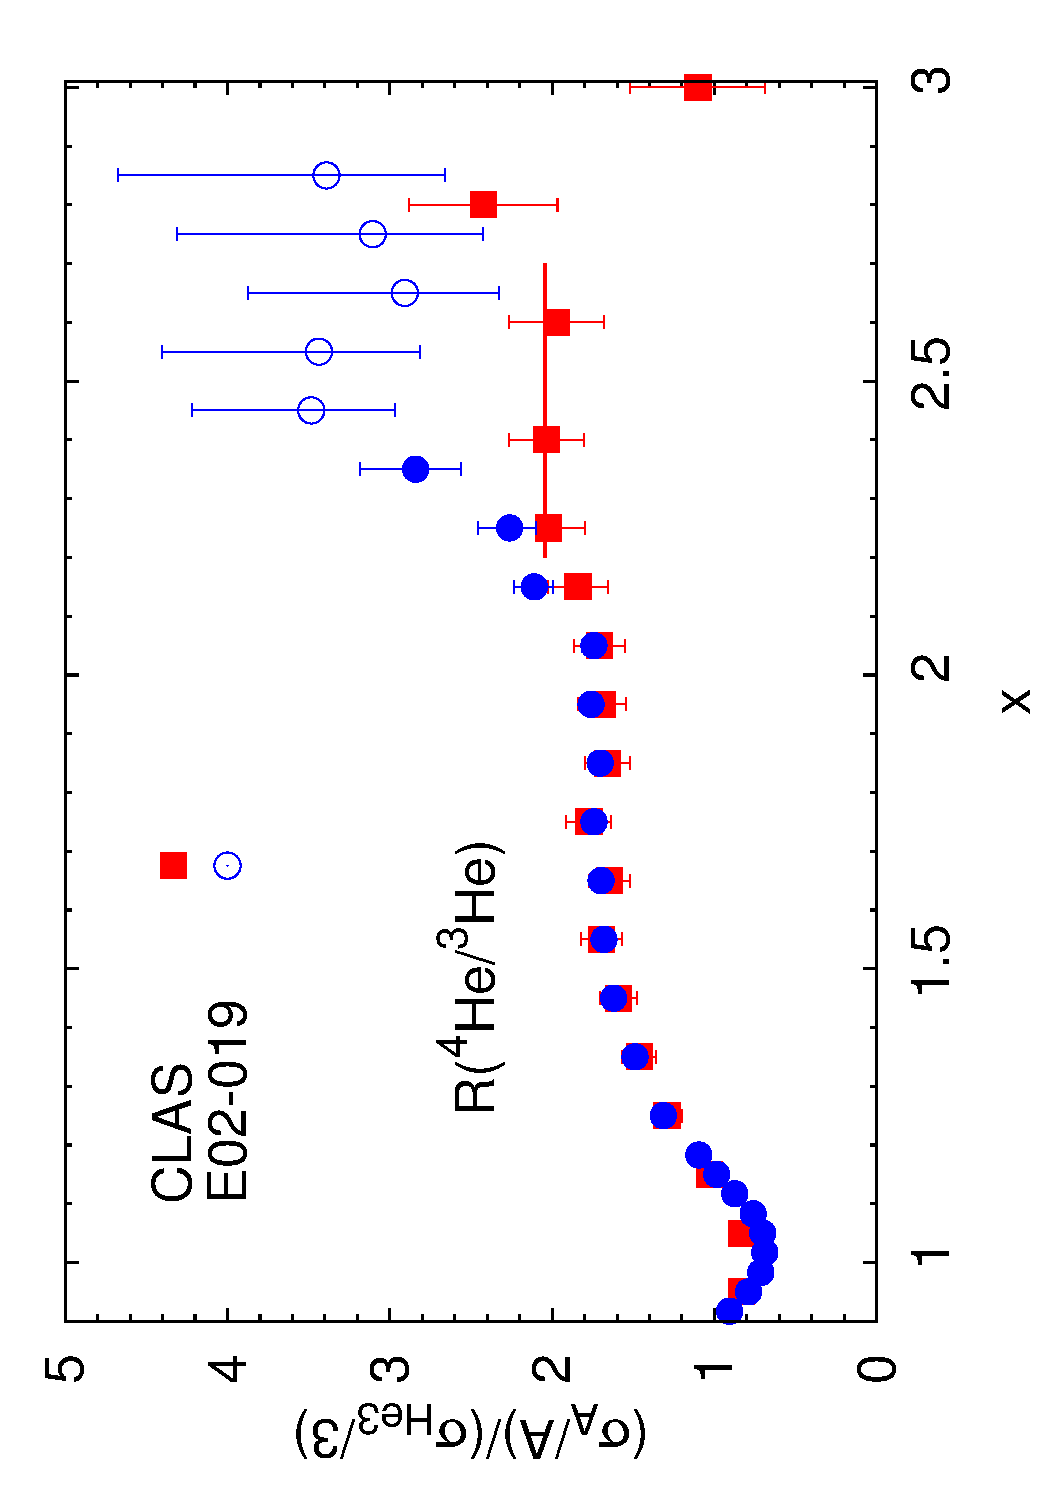
\includegraphics[type=pdf,ext=.pdf,read=.pdf,width=0.60\linewidth]{./figures/physics/E02019_2NSRC_3NSRC}
    \caption[2N-SRC and 3N-SRC results from E02-019 in Hall C]{\footnotesize{2N-SRC and 3N-SRC results from E02-019 in Hall C~\cite{PhysRevLett.108.092502} comparing with the result from Hall-B, where the blue dots are the E02-019 data and red dots are the CLAS data.}}
    \label{E02019_2NSRC_3NSRC}
  \end{center}
\end{figure} 

The other important study of SRCs in inclusive measurements is the difference of two scaling variables, $x_{bj}$ and $\alpha_{i}$. From Eq~\eqref{alpha_xbj}, the LC variable $\alpha_{i}$ is approximately equal to $x_{bj}$ at large $Q^{2}$. At low $GeV^{2}$, the approximation is not valid and the difference of the scaling behaviour in SRCs as a function of $x_{bj}$ or $\alpha_{i}$ is required to be carefully examined. 
\begin{figure}[!ht]
  \begin{center}
    \includegraphics[type=pdf,ext=.pdf,read=.pdf,width=0.60\linewidth]{./figures/physics/SLAC_2NSRC_xbj_alpha}
    \caption[Ratio of $^{56}Fe/^{2}H$ as a function of $x_{bj}$ and $\alpha_{2N}$]{\footnotesize{Ratio of $^{56}Fe/^{2}H$ as a function of $x_{bj}$ (left) and $\alpha_{2N}$ (right) for different $Q^{2}$ values~\cite{SLAC_Measurement_PRC.48.2451}, which shows that the LC variable provides better scaling behaviour.}}
    \label{SLAC_2NSRC_xbj_alpha}
  \end{center}
\end{figure} 
Although $\alpha_{i}$ can not be reconstructed in inclusive scattering, one can assume that in PWIA the virtual photon interacts with the nucleon in an 2N-SRC at rest. This assumption leads to a new expression of the LC variable specifically for 2N-SRC:
\begin{equation}
  \alpha_{2N} = 2-\frac{q_{-}+2m}{2m}\frac{\sqrt{W^{2}-4m^{2}}+W}{W},  
\end{equation}
where $q_{-}$ is the initial longitudinal momentum of the struck nucleon and $W^{2}=4m_{N}^{2}+4m_{N}\nu-Q^{2}$. The analysis of SLAC data~\cite{SLAC_Measurement_PRC.48.2451} reveals that $\alpha_{2N}$ can better isolate 2N-SRCs (Fig.~\ref{SLAC_2NSRC_xbj_alpha}) and allows one to examine the transition region from 2N-SRC to 3N-SRC. A more general expression for all $\alpha_{i}$ in the inclusive measurement can be obtained from~\cite{e08014_pr}:
\begin{equation}
  q_{-}\cdot\alpha_{jN}m_{N}+q_{+}\cdot\left(M_{A}-\frac{M_{r}^{2}}{m_{N}(j-\alpha_{jN})}\right)=m_{N}^{2},
\end{equation}
where $j=2,3,...$, $q_{+}$ is the initial transverse momentum of the struck nucleon and $M_{r}$ is the mass of the residual system. Taking $j=3$ can solve for $\alpha_{3N}$ but the exact expression depends on the value of $M_{r}$ since 3N-SRC has much more complicated configuration. As discussed in previous section, 3N-SRC-I is the dominant configuration in 3N-SRC where $M_{r}=2m_{N}$, and give:
\begin{equation}
  \alpha_{3N} = \frac{3}{2}+\frac{1}{2}[\sqrt{ (3+b_{1})^{2}-b_{2}}-b_{1}]
\end{equation} 
where,
\begin{equation}
  b_{1} = \frac{q_{+}}{q_{-}} \frac{M_{A}}{m_{N}}-\frac{m_{N}}{q_{-}},\qquad b_{2} = 16 \frac{q_{+}}{q_{-}}.
\end{equation} 
The value of $M_{r}$ becomes higher for non-parallel configuration, such as 3N-SRC-II. Examining the scaling as a function of $\alpha_{3N}$ and varying the value of $M_{r}$ provides a sensitive probe to the detailed structure of 3N-SRC~\cite{e08014_pr}.

%%%%%%%%%%%%%%%%%%%%%%%%%%%%%%%%%%%%%%%%%%%%%%%%%%%%%%%%%%%%%%%%%%%%%%%%%%%%%%%%%%%%%%%%%%%%%%%%%%%%%%%%%%5
%%%%%%%%%%%%%%%%%%%%%%%%%%%%%%%%%%%%%%%%%%%%%%%%%%%%%%%%%%%%%%%%%%%%%%%%%%%%%%%%%%%%%%%%%%%%%%%%%%%%%%%%%%%
%\section{Other Experiment Techniques}
\subsection{Semi-Inclusive and Triple-Coincidence Measurements}
\begin{figure}[!ht]
  \begin{center}
    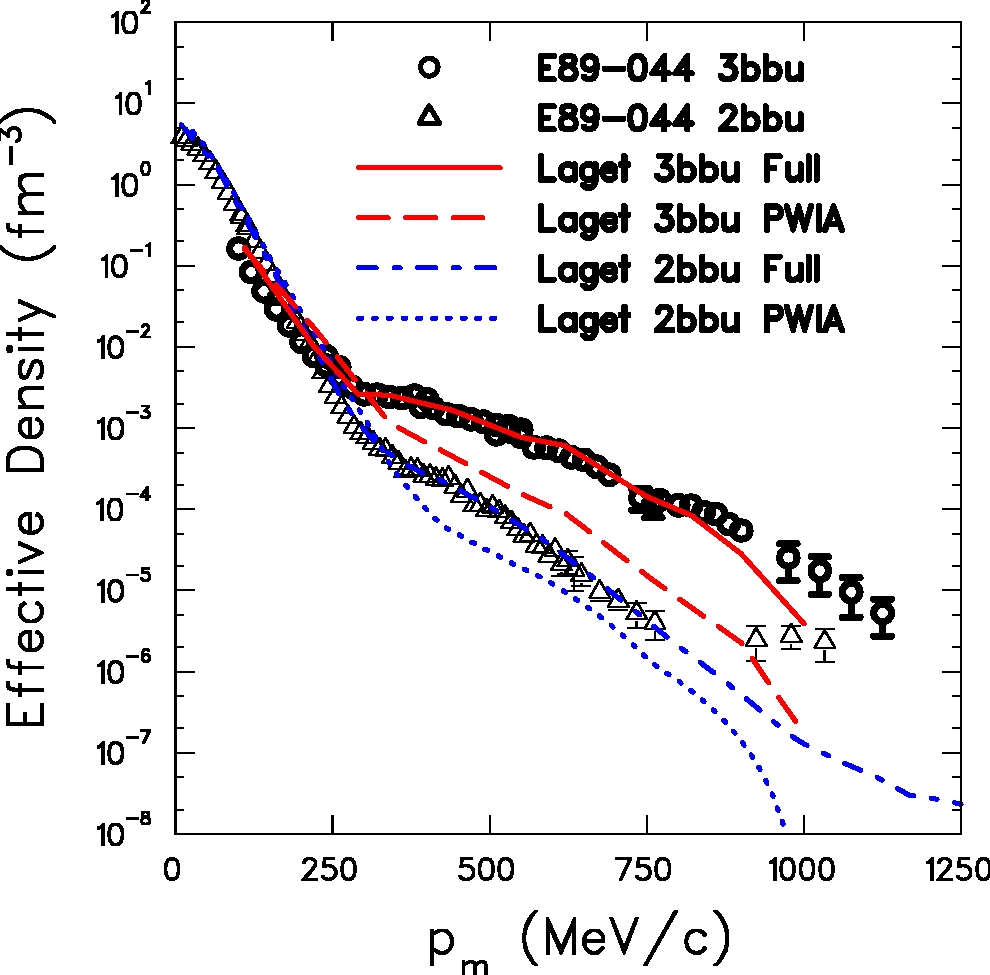
\includegraphics[type=pdf,ext=.pdf,read=.pdf,width=0.60\linewidth]{./figures/physics/10yrSRC_fig3}
    \caption[Proton Effective Momentum distribution in $^{3}He$.]{\footnotesize{Proton Effective Momentum distribution in $^{3}He$~\cite{PhysRevLett.94.082305}, where circles and triangles are experimental data in $^{3}He(e,e'p)pn$ three-body break-up and $^{3}He(e,e'p)d$ two-body break-up, respectively. Lines are theoretical calculations from~\cite{Laget200549}. For the missing momentum above the Fermi momentum (250 MeV), the momentum distribution of three-body break-up is much stronger than the one of two-body break-up, indicating the dominance of SRCs in this region.}}
    \label{10yrSRC_fig3}
  \end{center}
\end{figure} 
Proton-knock-out experiments allow the direct access of the proton's initial momentum distribution through the reconstruction of the nuclear spectral function from the exclusive cross sections. In addition to measuring the scattered electron, one can map out the effect of SRCs to the high momentum tail by detecting the struck proton. Since the correlated nucleon in 2N-SRC is ejected on the opposite direction is not detected, one generally treats the $A(e,e'p)$ reaction as semi-inclusive process. 

To evaluate the deviation of a theoretical calculation of the momentum distribution to the experimental cross section, a normalization factor is introduced in Eq~\eqref{quasi_xs_spectral_function} (for only one proton case)~\cite{Higinbotham:2009hi}:
\begin{equation}
  \frac{d^{6}\sigma}{(dEd\Omega)_{e}(dEd\Omega)_{p}} = K\sigma_{ep}S(E_{0},\mathbf{p_{0}})T_{A}(Q^{2}),
\end{equation}
where $K$ is a kinematic factor and the transparency, $T_{A}$ is the probability that a nucleon will be emitted from the nucleus with other effects, such as FSI. Experiments in Hall-C~\cite{PhysRevLett.80.5072,PhysRevC.66.044613,PhysRevC.72.054602} measured the values of $T_{A}$ for several nuclei which were found to be larger than the predictions in IPSM. Such an enhancement is mainly due to the SRCs effect~\cite{Higinbotham:2009hi}. 

Hall-A experiments ~\cite{PhysRevLett.94.082305,PhysRevLett.94.192302} studied the momentum distribution of $^{3}He$ and observed that the strength greatly increases in the high momentum tail compared with the expected strength including SRCs (Fig.~\ref{10yrSRC_fig3}). This scenario is explained as the combination of SRCs and FSI. 

%\subsection{Triple-Coincidence Measurements}
The exclusive cross section measurement of the $A(e,e'pN)$ reaction, or called the triple-coincidence experiment~\cite{PhysRevLett.90.042301,PhysRevLett.99.072501,src_since}, is able to direct probe the scattered electron, the struck nucleon and the spectator nucleon in 2N-SRC. Such an experiment not only can directly conform the production of 2N-SRC, but also can study the types of the nucleon pairs involved in the correlation.  
\begin{figure}[!ht]
  \begin{center}
    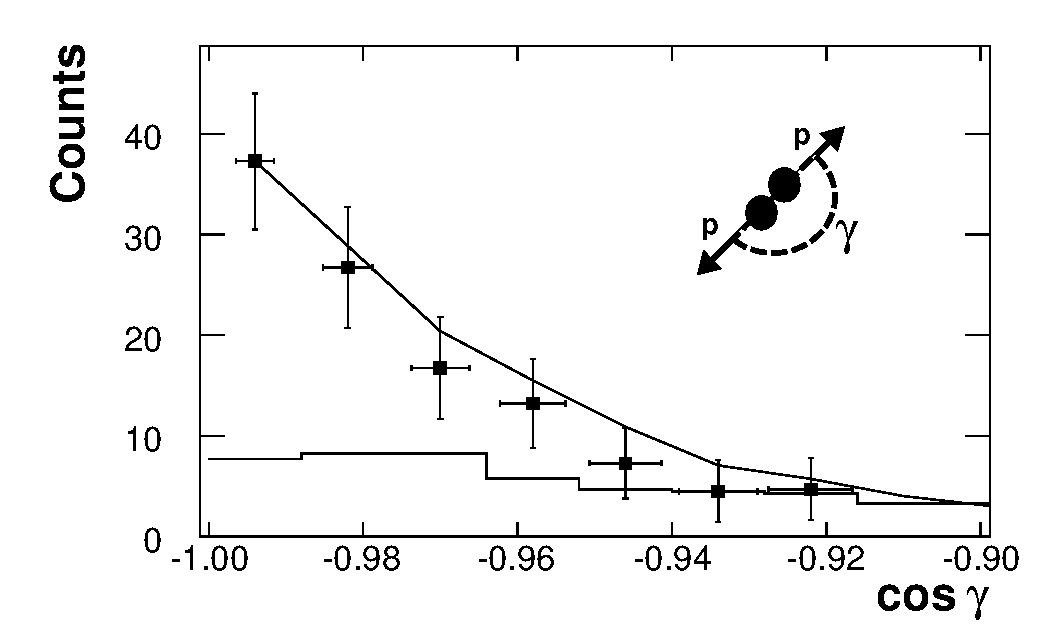
\includegraphics[type=pdf,ext=.pdf,read=.pdf,width=0.60\linewidth]{./figures/physics/10yrSRC_fig5}
    \caption[Angular correlation between nucleons in 2N-SRC]{\footnotesize{Angular correlation between nucleons in 2N-SRC, where the x-axis is the cosine of the opening angle between the struck nucleon and the spectator nucleon in the $^{12}C(e,e'pp)$ reaction~\cite{PhysRevLett.99.072501}.}}
    \label{triple_src_cos}
  \end{center}
\end{figure} 

A recent experiment in Hall-A, E01-015, ~\cite{PhysRevLett.99.072501,src_since}, has performed such a measurement using electron scattering on carbon target. In the $^{12}C(e,e'pp)$ reaction, the experiment studied the angular correlations between the struck proton and the spectator nucleons. Fig.~\ref{triple_src_cos} gives the distribution of the events in $cos\gamma$ when $p_{m}$=500~MeV/c, which clearly peaks near $cos\gamma=-1$. This result proved that the correlated nucleons are ejected back-to-back from the nucleus. The ratio of $pn$ and $pp$ in 2N-SRC can be extracted by using comparing $^{12}C(e,e'pp)$ and $^{12}C(e,e'pn)$. Fig.~\ref{triple_src_np} shows that the ratio of $np/pp$ pairs is around $18\pm 5$, which conforms that the 2N-SRC is dominated by the two-body tensor interaction. 
\begin{figure}[!ht]
  \begin{center}
    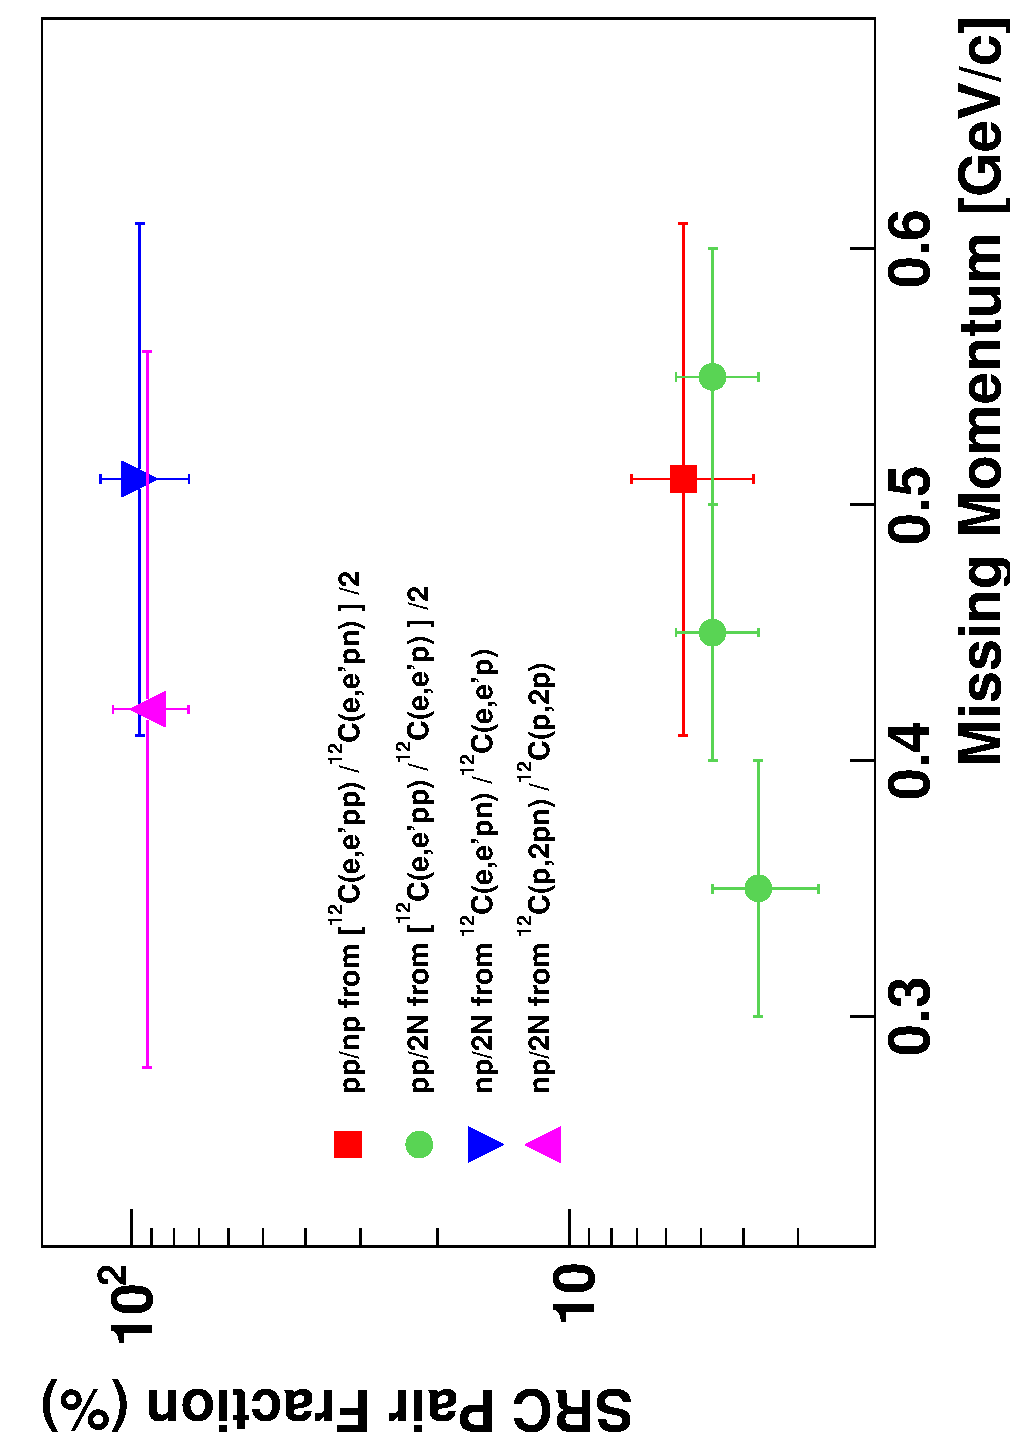
\includegraphics[type=pdf,angle=270,ext=.pdf,read=.pdf,width=0.60\linewidth]{./figures/physics/10yrSRC_fig7}
    \caption[The fraction of $np$ pairs to $pp$ pairs in 2N-SRC]{\footnotesize{The fraction of $np$ pairs to $pp$ pairs in 2N-SRC in carbon from the triple-coincidence experiment in Hall-A~\cite{src_since}.}}
    \label{triple_src_np}
  \end{center}
\end{figure} 

\section{Final State Interaction}
\begin{figure}[!ht]
  \begin{center}
    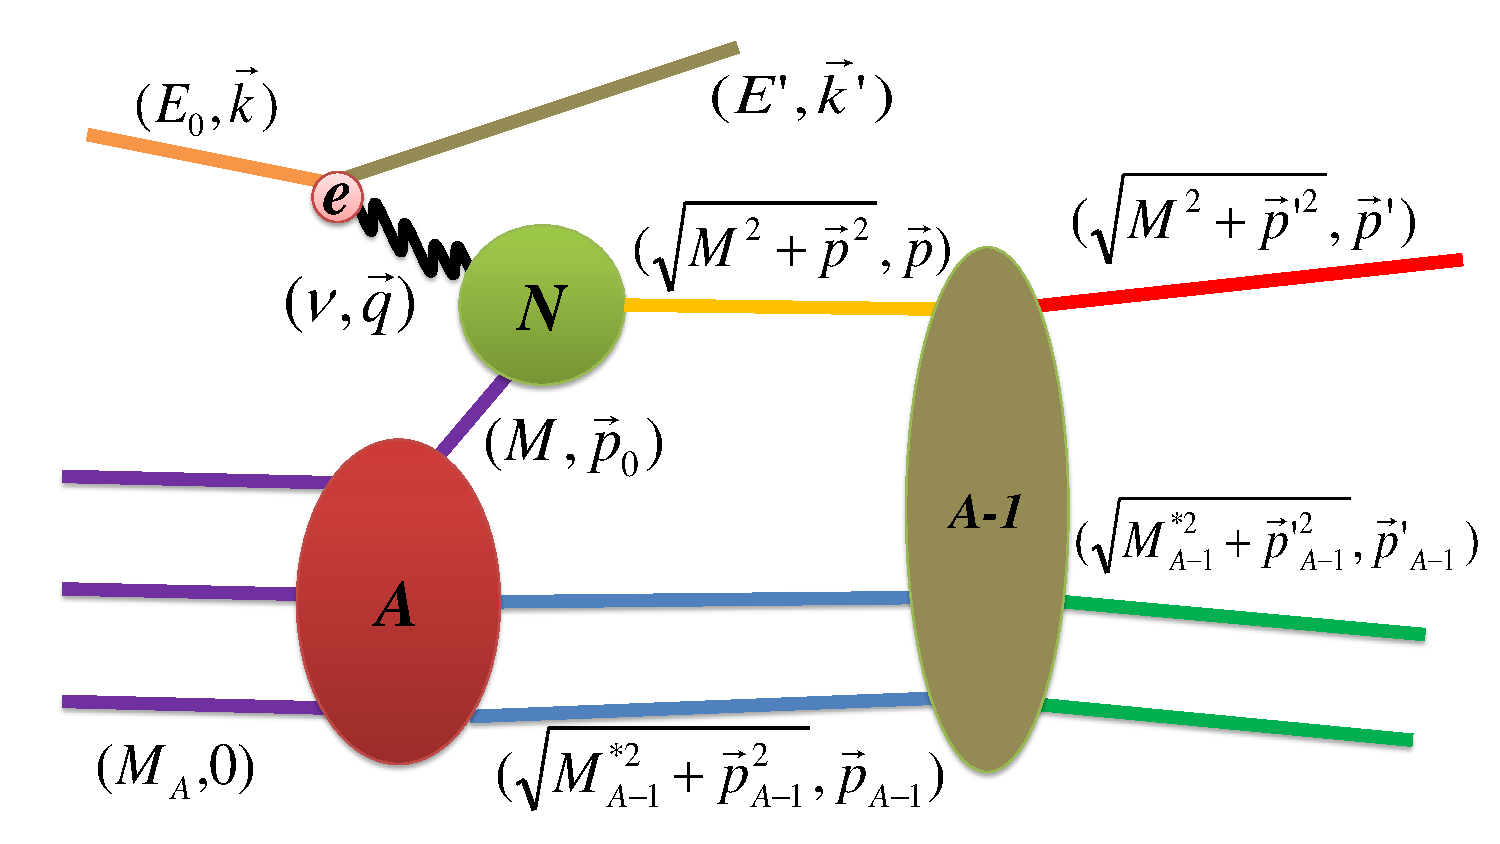
\includegraphics[type=pdf,ext=.pdf,read=.pdf,width=0.80\linewidth]{./figures/physics/FSI}
    \caption[Final state interaction]{\footnotesize{General diagram of final state interaction. The struck nucleon is re-scattered by the $A-1$ system and its final momentum is modified.}}
    \label{fsi}
  \end{center}
\end{figure}
Final State Interaction (FSI) is the effect of the struck nucleon being re-scattered by the $A-1$ recoil system. In PWIA, the nucleons in the nucleus are treated as individual constituents and the space resolution of the electron probe is approximately $1/q$. Hence, in the inclusive cross section measurement at large $Q^{2}$, FSI is negligibly small, based on the fact that the interaction time between the virtual photon and the struck nucleon is significant smaller than the one between the struck nucleon and the recoil system.

However, comparison between the theoretical calculation and experimental results~\cite{PhysRevC.46.1045,PhysRevC.87.024606} shows the violations of y-scaling for heavy target which indicates FSI still plays a significant role in the scattering process even at large $Q^{2}$.
(MORE discussion)

The effect of final state interaction (FSI) is proportional to $1/Q^{2}$. At low $Q^{2}$ the contribution of FSI is large enough to break down the y-scaling feature of quasi-elastic scattering in PWIA~\cite{Day:1987az}. The study of SRCs using inclusive cross section measurement requires sufficient $Q^{2}$ values to eliminate the FSI contribution. The current results of inclusive data (i.e. in Fig.~\ref{SLAC_2NSRC_xbj_alpha}) indicate no dependence of $Q^{2}$ for the scaling region of 2N-SRC, which proves that in the kinematic settings of SRCs study ($Q^{2}>1~GeV^{2}$) FSI has very small contributions.

The argument above is valid since the SRCs configurations are weakly interacting with other components in the nucleus and PWIA in the inclusive measurement is still applicable. However, the contribution of FSI within the SRC may not vanish even at very large $Q^{2}$. When the electron scattering on the nucleon in SRCs, the struck nucleon stays very close to other correlated nucleons and the probability of rescattering from the residual system is large. Despite the possible large contributions, FSI is localized in the SRCs and its contribution can be removed by taking the cross section ratio. For example, the FSI contribution in the 2N-SRC pairs in heavy nuclei should be similar to one in $^{2}H$, and the ratio, $\sigma_{A}/\sigma_{^{2}H}$, should be able to cancel the FSI effect and only yields the clean contribution from 2N-SRC. 

\section{E08014 Experiment}
\begin{figure}[!ht]
  \begin{center}
    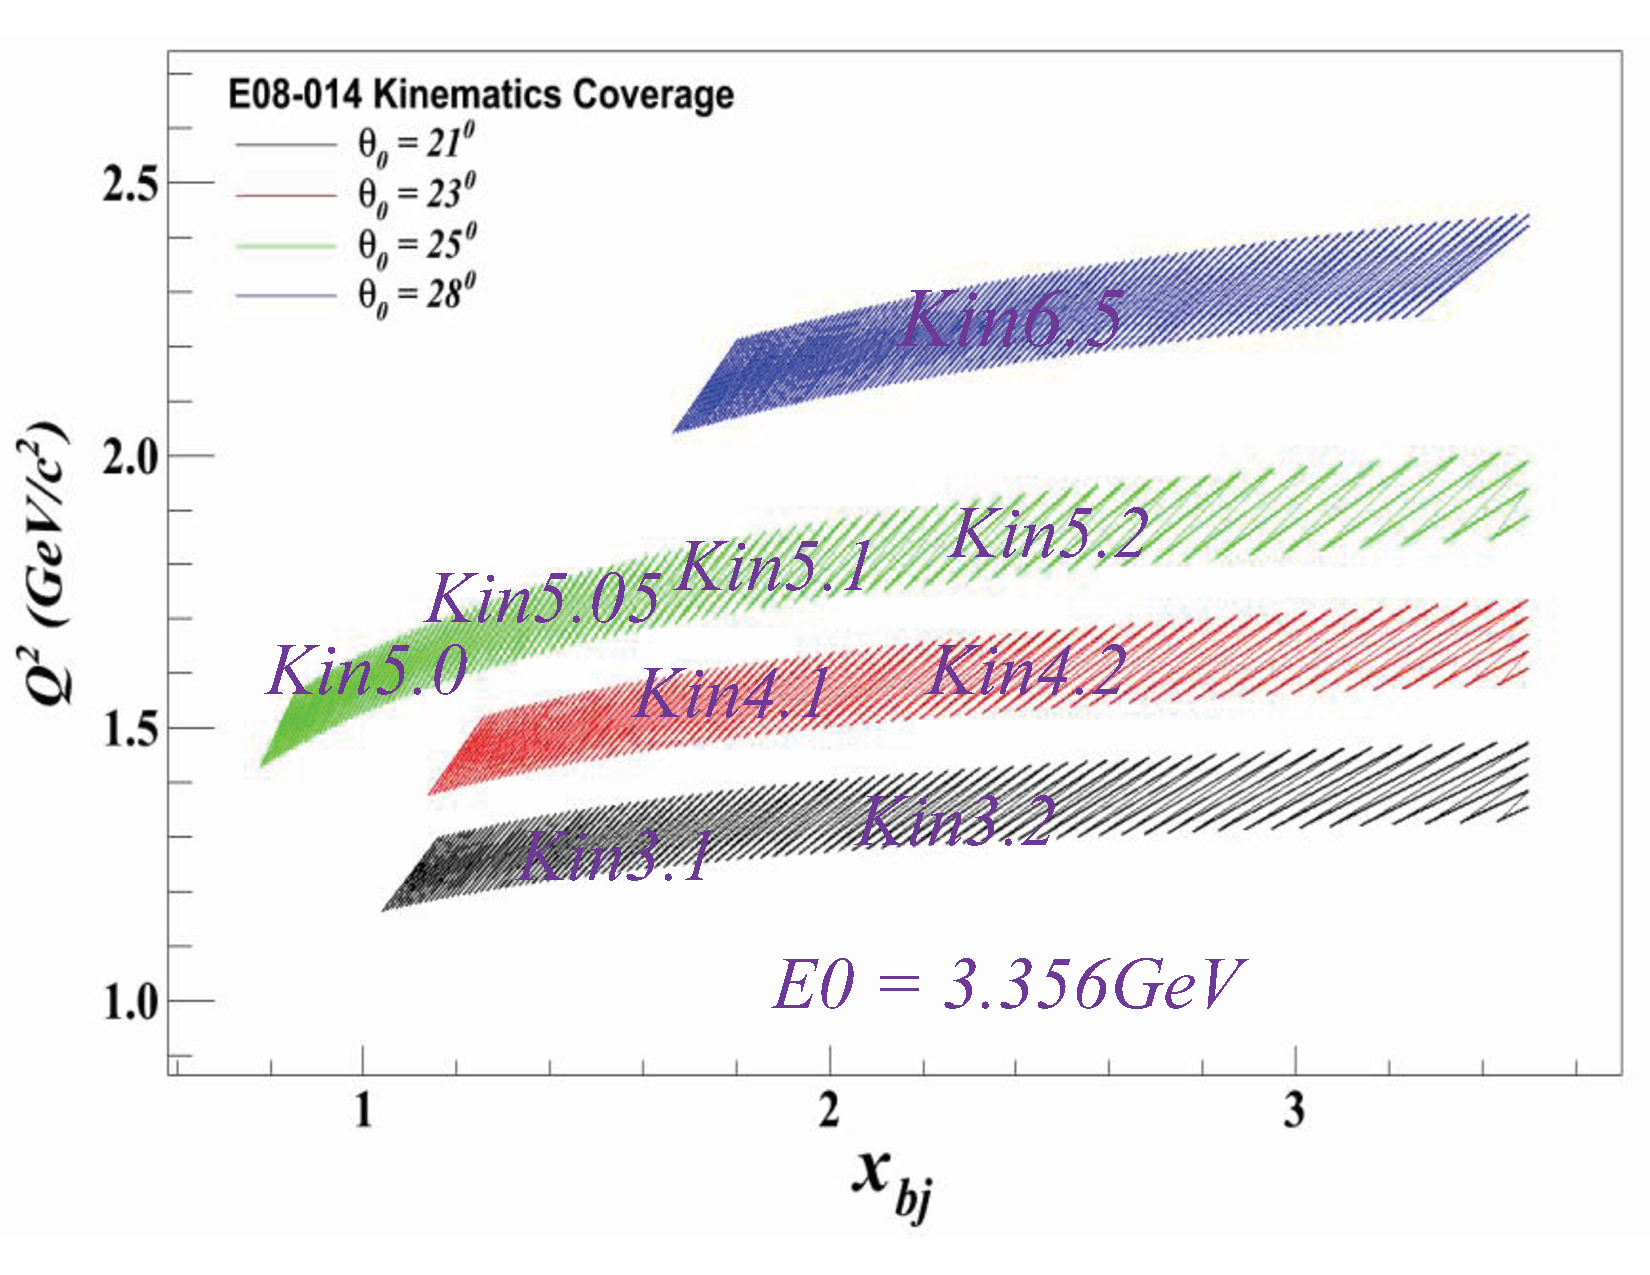
\includegraphics[type=pdf,ext=.pdf,read=.pdf,width=0.60\linewidth]{./figures/physics/E08014_Kin_Cover}
    \caption[Kinematic Coverage of E08-014 experiment]{\footnotesize{Kinematic Coverage of E08-014 experiment.}}
    \label{kin_cor}
  \end{center}
\end{figure}
An new experiment, E08-014~\cite{e08014_pr}, had been carried out in 2011 in Hall-A at Jefferson Lab, with electron beam energy of $3.356 GeV$ from the continuous electron beam accelerator facility (CEBAF). Utilizing the high resolution spectrometers in their standard configurations, as shown in Fig.~\ref{kin_cor}, this experiment measured the inclusive cross section of $^{2}H$, $^{3}He$, $^{4}He$, and $^{12}C$ at $1.1<Q^{2}<2.5 (GeV/c)^{2}$, which covers the range of $x_{bj}$ from the quasi-elastic peak region to above $3.0$. The absolute cross section results will be used to study the scaling function and momentum distribution at larger missing momentum, as well the effect of FSI. By taking the cross section ratio of heavy targets to $^{2}H$ or $^{3}He$, one can examine the $x_{bj}$ and $Q^{2}$ dependence and SRCs, and measure the values of $a_{2}$ and $a_{3}$. The relatively low $Q^{2}$ setting allows the study of $\alpha_{2N}$ and $\alpha_{3N}$ in the scaling of SRCs. The Calcium isotopes, $^{40}Ca$ and $^{48}Ca$, were also used to study the isospin dependence of 2N- and 3N-SRC. Detailed experiment setup and data analysis will be discussed in this thesis and preliminary results will also be presented. 
